\documentclass[a4paper,11pt]{article}

%%%%%%%%%
%%usees%%
%%%%%%%%%
\usepackage[utf8]{inputenc}
%\usepackage[ngerman]{babel}
%\usepackage{a4wide}
\usepackage[margin=3.0cm, top=3.0cm, bottom=3.0cm]{geometry}
\usepackage{setspace}
\usepackage{graphicx}
\usepackage{amssymb} 
\usepackage{amsmath}
\usepackage{mathtools}
\usepackage{footnote}
\usepackage{caption}
\usepackage{color}
\usepackage[hidelinks]{hyperref}
\usepackage{cite}
\usepackage{todonotes}
\usepackage{subfigure}
\usepackage{siunitx}
\usepackage{tabularx}
\usepackage{wrapfig}
\usepackage{url}
\usepackage{listings}


\newcommand{\reffig}[1]{Figure~\ref{#1}}
\newcommand{\refsec}[1]{Section~\ref{#1}}
\newcommand{\refdef}[1]{Definition~\ref{#1}}
\newcommand{\reflst}[1]{Listing~\ref{#1}}
\newcommand{\reftab}[1]{Table~\ref{#1}}

\definecolor{Mulberry}{cmyk}{0.34,0.90,0,0.02}
\definecolor{BrickRed}{cmyk}{0,0.89,0.94,0.28}
\lstset{language=C++,frame=none, basicstyle=\tt}
\lstdefinelanguage{CLIPS}{
  keywordsprefix=?,
  %keywordsprefix=\$,
  alsoletter={?=-<>*\$},
  keywordstyle=\color{Mulberry!80!black}\bfseries,
  keywords=[2]{deffunction, deftemplate, defrule, deffacts, defgeneric,
    defmodule, defadvice, defglobal, defmethod, definstance, defclass},
  keywordstyle=[2]\color{BrickRed!70!blue}\bfseries,
  keywords=[3]{slot, multislot, type, default, default-dynamic,
                      extends, crlf, range, nil, if, then, else, while,
                      not, or, switch, case, and, reset,
                      assert, test, declare, salience, return, bind, modify,
                      retract, explicit, unique, node-index-hash,
                      halt, printout, =>, <-},
  keywordstyle=[3]\color{darkgray}\bfseries,
  keywords=[4]{subsetp,progn, progn$, not, node-index-hash, create$,
    append$, length$, printout},%
  keywordstyle=[4]\color{gray}\bfseries,
  %identifierstyle=\color{black},
  sensitive=false,
  comment=[l]{;},
  commentstyle=\color{purple}\ttfamily,
  stringstyle=\color{red}\ttfamily,
  morestring=[b]"
}


\lstdefinestyle{CLIPS}
{
  language=CLIPS,
  basicstyle=\footnotesize\ttfamily\vspace{0.2cm},
  breaklines=true,
  showstringspaces=false,
  %keywordstyle=\bfseries,
  %keywordstyle=\color{Mulberry},
  frame=lines,
  belowcaptionskip=-3pt,
  emphstyle=\itshape,
  numbers=left,
  stepnumber=1,
  backgroundcolor=\color{gray!10},
  rulecolor=\color{gray!80},
  fillcolor=\color{gray!10},
  framexleftmargin=16pt,
  xleftmargin=16pt,
  %stringstyle=\color{BitterSweet},
  stringstyle=\color{BrickRed},
  commentstyle=\color{BrickRed},
  escapechar=\%,
  % emph={getup, servo, depends_skills},
  %emphstyle=\underbar,
  %numbers=left,
  %stepnumber=1,
  %%stringstyle=\ttfamily, % typewriter type for strings
  %float,
  captionpos=b
}

\lstdefinestyle{SmallCLIPS}{
  style=CLIPS,
  basicstyle=\ttfamily\footnotesize,
  numbersep=6pt,
}
\lstdefinestyle{ReallySmallCLIPS}{
  style=CLIPS,
  basicstyle=\ttfamily\scriptsize,
  numbersep=5pt,
}

\lstdefinestyle{ReallySmallCLIPSNoFrame}{
  style=CLIPS,
  basicstyle=\ttfamily\scriptsize,
  numbersep=5pt,
  frame=none,
  backgroundcolor=\color{white},
  framextopmargin=0pt,
  framexbottommargin=0pt
}

\lstdefinestyle{SuperSmallCLIPSNoFrame}{
  style=CLIPS,
  basicstyle=\ttfamily\fontsize{10pt}{10pt}\selectfont,
  numbers=none,
  frame=none,
  backgroundcolor=\color{white},
  framextopmargin=0pt,
  framexbottommargin=0pt,
  framexleftmargin=-2pt, xleftmargin=-2pt,
}

\lstdefinestyle{SmallCLIPSNoFrame}{
  style=CLIPS,
  basicstyle=\ttfamily\footnotesize,
  numbersep=5pt,
  frame=none,
  backgroundcolor=\color{white},
  framextopmargin=0pt,
  framexbottommargin=0pt
}

\lstdefinelanguage{JavaScript}{
  keywords={typeof, new, true, false, catch, function, return, null, catch, switch, var, if, in, while, do, else, case, break},
  keywordstyle=\color{blue}\bfseries,
  ndkeywords={class, export, boolean, throw, implements, import}, %, this
  ndkeywordstyle=\color{darkgray}\bfseries,
  identifierstyle=\color{black},
  sensitive=false,
  comment=[l]{//},
  morecomment=[s]{/*}{*/},
  commentstyle=\color{purple}\ttfamily,
  stringstyle=\color{red}\ttfamily,
  morestring=[b]',
  morestring=[b]"
}

\lstdefinestyle{JSON}
{
  language=JavaScript,
  morekeywords={interface,field,message,comment},
  basicstyle=\footnotesize\ttfamily\vspace{0.2cm},
  breaklines=true,
  showstringspaces=false,
  %keywordstyle=\bfseries,
  keywordstyle=\color{Mulberry},
  frame=lines,
  belowcaptionskip=8pt,
  emphstyle=\itshape,
  numbers=left,
  stepnumber=1,
  backgroundcolor=\color{blue!10},
  rulecolor=\color{blue!50},
  fillcolor=\color{blue!20},
  framexleftmargin=16pt,
  xleftmargin=16pt,
  %stringstyle=\color{BitterSweet},
  stringstyle=\color{BrickRed},
  commentstyle=\color{BrickRed},
  escapechar=\%,
  % emph={getup, servo, depends_skills},
  %emphstyle=\underbar,
  %numbers=left,
  %stepnumber=1,
  %%stringstyle=\ttfamily, % typewriter type for strings
  captionpos=b
}

\lstdefinestyle{SmallJSON}{
  style=JSON,
  basicstyle=\ttfamily\footnotesize,
  numbersep=6pt,
}
\lstdefinestyle{ReallySmallJSON}{
  style=JSON,
  basicstyle=\ttfamily\tiny,
  numbersep=5pt,
}


%%%%%%%%%
%%Title%%
%%%%%%%%%

\author{Frederik Zwilling 304314}
\title{Master-Thesis Proposal:\\ Shared Robot Memory for Multiple Planners in Fawkes}
\begin{document}
%\thispagestyle{empty}
%\tableofcontents
%\newpage
%\onehalfspace
\maketitle
%%%%%%%%%
%%Text%%
%%%%%%%%

\abstract{abstract.}

\section{Introduction}
\label{sec:introduction}
\begin{itemize}
\item Motivation Knowledge Representation on Cyber Physical Systems
\item Problem description
  \begin{itemize}
  \item Worldmodel exchange between resoners/planners
  \item Worldmodel exchange between robots
  \item Long time storage
  \end{itemize}
\item Idea Robot Memory
\item Application RCLL PDDL-CLIPS
\item Application @Home/PR2
\end{itemize}

\section{Background}
\label{sec:background}
This section presents the background of the proposed thesis. On the
one hand, we describe the primary application and evaluation domain,
the RoboCup with the RoboCup Logistics League (RCLL), the @Home league
and their robots in ~\ref{sec:robocup}. On the other hand, we present
the most important software for the proposed thesis. In
section~\ref{sec:fawkes} we present the robot software framework
Fawkes. Section~\ref{sec:planners} describes the planners and
reasoners which should profit from using the robot memory and in
section~\ref{sec:mongodb} MongoDB, the database used in the backend of
the robot memory.

\subsection{RoboCup}
\label{sec:robocup}
\todo[inline]{rewrite or copy from bachelorthesis?}  The
\emph{RoboCup} is an international robotics competition founded to
foster research in the field of robotics and artificial
intelligence.~\cite{Robocup}. It provides standard problems as a
platform to foster and compare research results. Research
teams from all over the world compete in different leagues to
benchmark their robotic system. The RoboCup provides a research
test-bed, in which participating teams implement new approaches and
make them robust against the challenges of the real world
complexity. Furthermore, the competition leads to comparison and
evaluation of different approaches.\\
%
The RoboCup features a variety of leagues, each focusing on another
aspect or application domain of robotics and artificial
intelligence. The majority of the RoboCup leagues host soccer robots
in different sizes and complexities. The leagues range from the
\emph{Small Size League} with small cylindrical robots and ground
truth perception from an overhead camera to humanoid robots in teen
size which need to have all sensors and computation devices on the
robot. The RoboCup also features more application oriented domains,
e.g. the \emph{Rescue League} with robots solving different
challenges in desaster scenarios and \emph{RoboCup@Work} with robots
operating in an industrial scenario to perform identification,
handling and transporting tasks with work related objects such as
skrews and nuts. The \emph{RoboCup Logistics League (RCLL)} which
features logistics robots in a production scenario and the
\emph{RoboCup@Home} leage featuring service robots in a domestic
environment are presented in the following in more detail because
these two leagues are used as application and evaluation domains of
the proposed thesis.


\subsubsection{RoboCup Logistics League}
\begin{figure}
  \begin{minipage}[b]{0.5\linewidth}
    \centering
    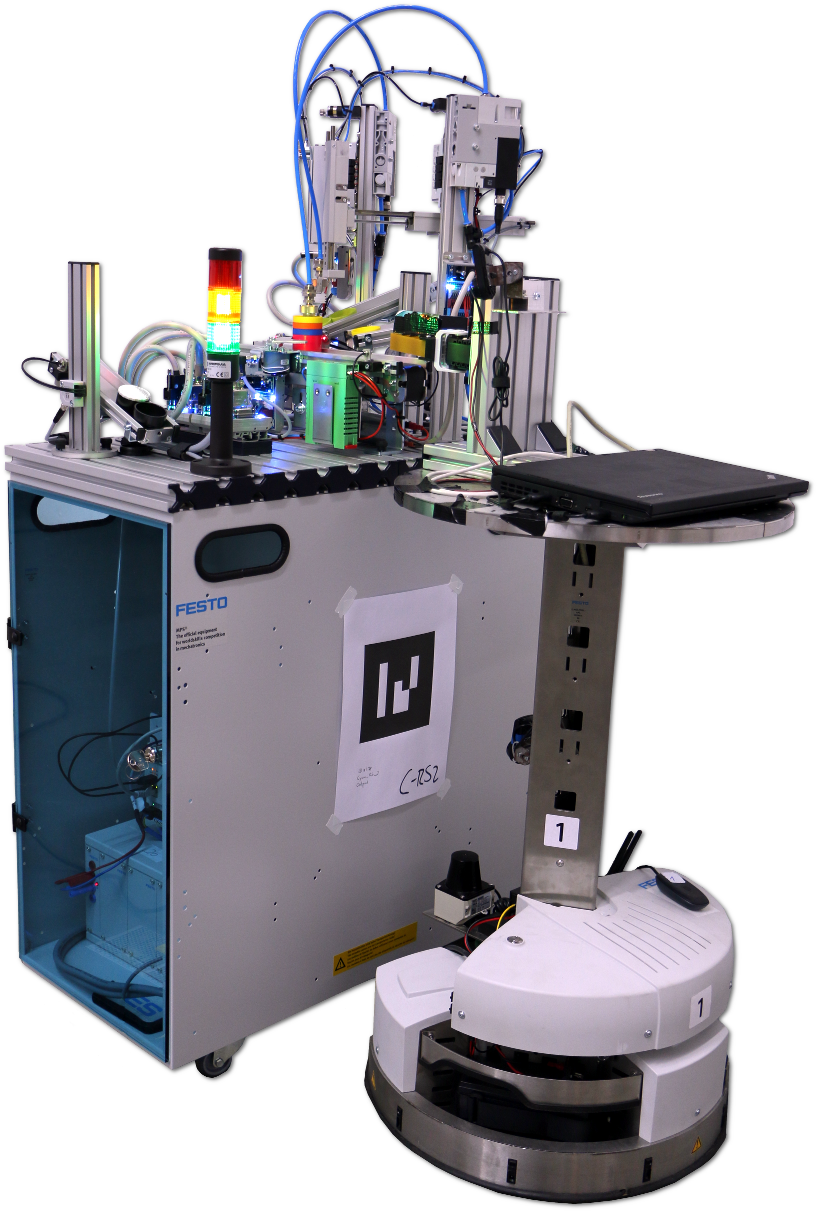
\includegraphics[width=0.5\textwidth]{img/rcll}
    \caption{Robot and MPS used in the RCLL}
    \label{fig:rcll}
  \end{minipage}
\quad
\begin{minipage}[b]{0.5\linewidth}
  \todo[inline]{empty}
  \label{fig:}
\end{minipage}
\end{figure}

\todo[inline]{League, robotino}
%
The \emph{RoboCup Logistics League (RCLL)}\footnote{RoboCup Logistics
  League website: \url{http://www.robocup-logistics.org}}, previously
LLSF, is a industry-oriented competition within RoboCup.  It tackles
the problem of production logistics in a smart factory where mobile
robots have to plan, execute, and optimize the material and production
flow between machines to produce and deliver products according to
dynamic orders. Competing teams deploy a group of up to three robots
which have to autonomously build ordered products by interacting with
\emph{Modular Production Machines (MPS)} and transporting workpieces
between these machines.  \reffig{fig:rcll} shows an RCLL robot filling
a machine which mounts colored rings on workpieces. The robots are
based on the Festo Robotino 3 platform which uses an holonomic drive,
and can be extended and programmed by the teams. The robot shown in
\reffig{fig:rcll} was build by the Carologistics team and used an
laser range finder for localization, a custom made gripper for
handling workpieces and several cameras for detection of AR-tags and
light-signals mounted on the machines~\cite{Carologistics2015}. The
game is controlled by a software component called \emph{referee box
  (refbox)} which randomizes the machine placement in the factory and
the production orders, communicates with the competing robots,
controls the machines and awards points.

The game consists of two phases~\cite{LLSF-Rules-2015}. In the first
phase, the \emph{exploration phase}, the robots have to roam the
factory to find randomly placed machines which are used later. By
detecting the light signal shown by the machines, the robots can
determine the machine-type. For correct reportsof discovered machines
to the refbox the team is awarded points, for incorrect ones points
are subtracted.
%
\begin{figure}[t]
  \centering
  \begin{minipage}{.8\linewidth}
  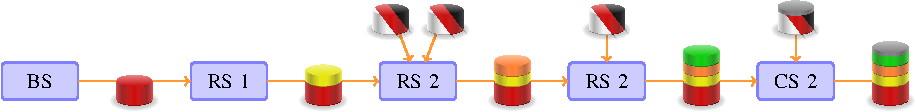
\includegraphics[width=\linewidth]{img/chain_c3}%
  \end{minipage}
  \quad%
  \begin{minipage}{.15\linewidth}
  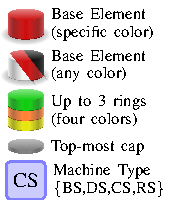
\includegraphics[width=\linewidth]{img/legend}%
  \end{minipage}
  \caption{Production chain of a high complexity
    product in the RCLL.}
  \vspace{-2mm}
  \label{fig:prod-chain}
\end{figure}
%
In the second phase, the \emph{produciton phase}, the refbox announces
orders, which products have to be produced by the robots. The products
are build from colored cups with optionally mounted rings and and a
colored cap. \reffig{fig:prod-chain} shows the production chain to
build a high complexity product. There are four different machine
types. The \emph{base-station (BS)} provides new bases, the colored
cups, as raw ressource. The \emph{ring stations (RS)} mounts colored
rings on a workpiece and after preparing it with a varying amount of
bases. The \emph{cap-station (CS)} mounts black or grey caps to finish
a product after loading it with a cap form a shelf first. The
\emph{delivery-station (DS)} is used to deliver products.

The challenges of the RCLL lie in the dynamic and only partially
observable environment the robots have to robustly and fully
autonomously work in, in the planning and multi-robot coordination
required to build as many ordered products as possible and deliver
them in time given time window, and in the baseline robotic challenges
such as collision avoidance, perception and behavior execution. The
dynamism of the environment is caused by the ranomized factory layout,
randomized out-of-order times of machines, the highly customizable
amount of products that preclude producing in advance, unknown
obstacles, such as the other teams robots and hard to completely avoid
handling mistakes by the robots. To cope with these challenges and
achieve an efficient production, a multi-robot decision making is
nesseccary.
\todo[inline]{Connection to robot memory}

\subsubsection{@Home League}


\begin{figure}[t]
  \centering
  \begin{minipage}{.6\linewidth}
    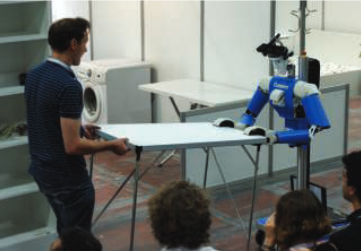
\includegraphics[height=120px]{img/athome-table}%
  \end{minipage}
  \quad%
  \begin{minipage}{.35\linewidth}
  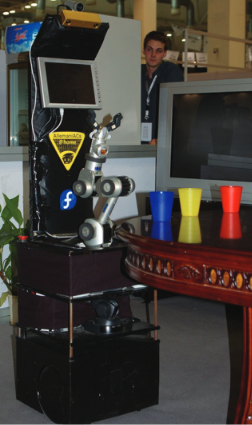
\includegraphics[height=120px]{img/ceasar}%
  \end{minipage}
  \caption{RoboCup@Home robot helping to carry a table
    (left)~\cite{athome-bit} and tidying up
    (right)~\cite{wisspeintner2009robocup}}
  \vspace{-2mm}
  \label{fig:athome}
\end{figure}

The RoboCup@Home league is a competition about domestic service
robots~\cite{wisspeintner2009robocup}. The robots have to assist
humans in a wide variety of everyday tasks. These tasks include
serving drinks, cleaning, setting tables, guiding or following people,
helping in emergency situations, shopping, cooking and
more. \reffig{fig:athome} shows two examples of @Home robots in the
competition.
%
The goal of the RoboCup@Home league is to foster and benchmark
research in the area of domestic service robots, to build a research
community and to envision autonomous multi-purpose robots helping
humans and especially elder people in the personal life.

The competition consists of an open challenge and multiple subtasks
such as finding and manipulating objects, navigation tasks,
remembering persons, wait on tables and acting as
nurse~\cite{athome-rules}. To solve these challenges, robots need to
have a wide variaty of abilities, including navigation, object
detection and manipulation, speech recognition and especially human
robot interaction, which requires, for example, applying everyday
knowledge to incomplete task descriptions given by humans.

Important challenges in the @Home league are acting robustly in a
dynamic and only partial observable domestic environment where people
and objects can disappear or be moved without the robot recognizing
it. Furthermore, detecting and manipulating objects in a personal
environment can be difficult because the space the robot acts in, for
example the frige, can be very clouded.

\todo[inline]{connection robot memory}

\subsection{Fawkes Robot Software Framework}
\label{sec:fawkes}
The basis for the proposed thesis is the robot software framework
\emph{Fawkes}\footnote{\url{http://www.fawkesrobotics.org}}. It is
available as Open Source and developed at the Knowledge-based Systems
Group\footnote{\url{http://www.kbsg.rwth-aachen.de}} (KBSG) at RWTH
Aachen University~\cite{FawkesDesign}. It is designed to work with a
plenthora of robots in different domains and follows a component-based
software design which separates functional entities into individual
software modules~\cite{component}. This enables reusing common
software solutions for robotic problems such as localization,
navigation, perception, reasoning and behavior execution. The binary
components can be loaded as \emph{plugins} at run-time.
%
Plugin activity is organized in threads to make use of multi-core
architectures. The threads can be run continously ore be hooked into
the main-loop of Fawkes to order the execution into a
\emph{sence-think-act} cycle to guararnee that higher-level components
can use the latest data. Furthermore, Fawkes guarantees loop times by
monitoring and eventually pausing and resuming threads running for too
long in one loop iteration.
% Ros blabla from BA?
Features in Fawkes are provided as \textit{aspects}. These aspects are
based on aspect-oriented programming~\cite{aspect_oriented} and give
access to a particular feature. Threads that want to use a feature can
inherit from the corresponding aspect. For example there are aspects
for accessing the blackboard, logging and timing~\cite{tnthesis}.

The communication between plugins is realized with a \emph{blackboard}
paradigm. The blackboard lists structured entries called
\emph{interfaces} which contain informaiton. Interfaces can be
provided by one plugin at a time, the writer, and read by other
plugins, the readers. This allows a very flexible communication
because the information provision in the interface is decoupled from
the concrete components which use the information and plugins writing
to the interfaces can be exchanged, e.g. by simulation plugins writing
to the same interface. Furthermore, the blackboard architecture
simplifies debugging because the current communication between two
plugins, determined by the state of the interface, can be viewed and
logged at runtime. To send commands to an interface writer, e.g. a
motor command to the motor controller, readers can send messages to
the interface.

As a communication infrastructure between different components, the
blackboard is one possibility to realize a robot memory shared between
multiple planners and reasoners in the current version of
Fawkes. Indeed the blackboard works well for providing information and
sending commands, though there are major limitations for this
application. One limitation is the strict rule, that only one
component can write an interface to provide information. This rule is
very usefull to avoid problems in standart plugin communication but
obstructive for multiple components sharing common information. For
example when a reasoner concludes that a product is placed at the
machine output after the production time and a behavior execution
component concludes that the robot holds the product after the grabing
action succeded, both components would have to modify the same piece
of information in the shared robot memory. Another limitation is the
fixed size and structure of blackboard interfaces. Therefore it is not
possible to dynamically represent more information, such as positions
of detected objects, than initially defined. Furthermore, the blackboard
does not support long-time memory.

\subsection{Planners and Reasoners}
\label{sec:planners}
This subsection gives an overview of planners and reasoners which are
going to profit from using and communicating with the robot
memory. For the variety of these, we give three\todo{four?} concrete
examples which should use the robot memory to achieve new or improved
functionality and to evaluate this thesis. The example planner and
reasoner systems are \emph{CLIPS}, a rule-based production system,
\emph{Golog}, a high-level programming language based on the Situation
Calculus, and the \emph{Planning Domain Definition Language (PDDL)},
which incorporates a family of planning formalisms into a standart
programming language. These examples are representatives for often
used types of planners and reasoners. However, the robot memory should
not be limited to these examples and provide a general C++ interface.

\subsubsection{CLIPS rules engine} The reasoner we currently use in the RCLL
to implement the high-level game agent is the rule-based production
system CLIPS which uses forward chaining based on the Rete
algorithm~\cite{Rete}. CLIPS consists of a fact-base, which is a
working memory with many small pieces of information, a knowledge base
with rules and procedures, and an inference engine~\cite{CLIPS-RM}
working with the knowledge base on the fact-base. The pieces of
information in the fact-base are called facts and consist of a name
and a key-value structure defined in a template for \emph{unordered
  facts}
(e.g. \textit{(position~(name~robot1)~(translation~2.5~1.0~0.0)}) or
an ordered list of values for \emph{ordered facts}.
\begin{figure}
\begin{lstlisting}[showlines,style=ReallySmallCLIPS, caption={CLIPS
    rule to change a robots state when the object it searched for is visible.},
  label=lst:clips-rule,
  emph={skill, args, state, target, res},
  emphstyle=\bfseries\color{green!80!black},
  emph={[2]\?skill, \$\?args, wait-for-lock, \?target, use,
  WAIT-FOR-LOCK, SKILL-EXECUTION, running},
  emphstyle={[2]\bfseries\color{blue!80!black}},
  morekeywords={retract, assert, modify, skill-call, skill-to-execute,
  wait-for-lock}]
(defrule found-machine
  ?s <- (state SEARCHING_FOR ?machine)
  (visible  (name ?machine))
  (position (name robot1) (translation $?pos))
  =>  
  (retract ?s) 
  (assert (state IDLE))
  (printout t "Found machine " ?machine " at " ?pos crlf)
)
\end{lstlisting} %$ This is just to fix Emacs highlighting due to dollar sign in code above
\end{figure}
An example rule is shown in \reflst{lst:clips-rule}. Rules are
composed of an \emph{antecedent} and a \emph{consequent}. The
antecendent is written before $=>$ and describes the contition that
has to be satisfied before the the rule is activated. It consists of a
list of patterns that have to be matched by the fact-base. For the
antecendent in \reflst{lst:clips-rule} there have to be fitting
\textit{state}, \textit{visible}, and \textit{position} facts where
$?$ and $\$?$ mark variables. The consequent is the part behind $=>$
and defines the procedure that is executed when the rule is
activated. It usually modifies the fact-base by retracting and
asserting facts as in the example to remove the old and add a new
state fact. The inference engine is responsible for checking which
rule antecendents are satisfied by the fact-base. If multiple rules
could fire, the inference engine chooses the rule with the highest
priority, executes the consequent and checks again. \emph{Functions}
can be called in the consequent, can have side effects and also be
implemented in C++. The RCLL agent implemented in CLIPS represents its
knowledge about the state of the world, the \emph{world model}, in its
fact-base. It controls which actions are taken by the robot by using a
technique called \emph{Incremental Reasoning}~\cite{CLIPS-Agent}. This
basically means that, whenever the robot is idle, it searches for the
next best task and executes it. For each task there is a rule with its
preconditions in the antecendent and the actions to take in the
consequent. There are also rules for modifying the worldmodel
(e.g. after finishing actions or getting new sensor data), task
execution, coordination with other robots and more. The coordination
of the robot team includes synchronizing their world model, so each
robot knows what other robots noticed and changed in the environment,
and resource allocation to ensure no two robots try to use the same
machine at a time or try to achieve the same goal by choosing a
redundant task. This coordination is currently implemented in CLIPS
rules using Profobuf\footnote{Google Protocol Buffers}
messages. Alternatively, this could also be done by using a
distributed robot memory which contains the world model in a
distributed database. This would be advantageous
because the database already provides efficient synchronization and
the implementation in CLIPS is not convinient due to its
specialization on logical rules.


\subsubsection{Planning Domain Definition Language (PDDL)} PDDL is a
standardized language for planning problems~\cite{PDDL}. It allows
modeling the nature and behavior of a domain as well as the
\emph{actions} possible to perform in a \emph{problem
  description}. With an additional \emph{problem description} which
defines the problem to solve it can be given to a PDDL planner which
searches for a totally or partially ordered sequence of actions, the
\emph{plan}, to solve the problem.
%
\todo[inline]{action example}
%
\reflst{lsf:pddl-action} shows an example action contained in a domain
description. Actions consist of preconditions and effects.  There are
various versions and extensions of PDDL which introduce new concepts
and features. A version often used in RoboCup domains is
PDDL~2.1~\cite{PDDL2.1} \todo{really?}. It adds numeric values and
continous actions. This allows finding optimal plans in continous
environments where, for example, distances and travel times
matter. PDDl has the advantage of being able to find comlete and
optimal, or at least efficient, plans. However, this comes with the
drawbacks of high computational effort for larger domains and the
problem of adopting to events during plan execution. For example when
the domain is not fully observable, the robot could sense changes in
the environment or fail executing an action. This would require
notifying the planner, incorporating the changes in PDDL and
replanning. To solve this problem we want to combine PDDL with an
execution in CLIPS. Then PDDL generates an efficient and complete plan
with coarse actions and CLIPS executes the plan action for action,
while monitoring the execution and updating the worldmodel according
to percieved changes. This world model is written into the robot
memory so that PDDL can access the world model with all applied
changes. This way the strenghtes of both PDDL and CLIPS.


\subsubsection{Golog } Golog is a high-level programming language based on the
\emph{Situation Calculus}, a first order logic formalism for knowledge
representation and reasoning in dynamic domains~\cite{Golog}. It
allows representing world states as terms called
\emph{situations}. These can be used in relations and functions called
\emph{fluents}. (e.g. $holding(x,s)$ is a fluent representing if
object $x$ is hold by the robot in situation $s$.) \emph{Actions} can
lead to new situations (e.g. $s'=do(pickup(x),s)$) and are modeled
with \emph{precondition axioms} (e.g. $Poss(pickup(x),s) \equiv
\forall y [\neg holding(y,s)]$). The value of relational fluents after
performing actions is defined by \emph{successor state axioms}
(e.g. $Poss(drop(x),s) \supset [broken(x,do(a,s)) \equiv a=drop(x)
  \wedge fragile(x) \vee broken(x,s) \wedge \neg a=repair(x)]$).
Golog as a high-level programming laguage features imperative
programming constructs such as procedures, conditions and loops as
well as nondeterministic branching. There are multiple dialects of
Golog which add features needed for robotic
applications. ConGolog~\cite{ConGolog} adds concurrency and
interrupts, IndiGolog~\cite{IndiGolog} adds on-line execution of
programs and sensing actions, which determine the value of a fluent
during execution, and ReadyLog~\cite{ferrein08ras} extends IndiGolog
with passive sensing during the execution of other actions. With these
dialects, Golog has been proven as useful for robot applications in
multiple domains such as domestic service robots. By providing an
interface to the robot memory, the strengthes of Golog, the highly
expressive behavior specification, can be combined with other
approaches to compensate the weaknesses, e.g. unefficient
planning~\cite{Golog-Planning}. There already are approaches to
combine Golog an PDDL into a continous planning framework that uses
PDDL for planning and Golog for execution and expanding placeholder
actions into sub-plans based on current information unavailable during
initial planning~\cite{ContPlanGolog}. It is implemented with a
translation between PDDL and
Golog~\cite{Golog-PDDL-Trans}. Furthermore, the robot memory could be
useful as additional persistent and distributed knowledge storage
(e.g. for saving the context during an interrupt\todo{cite Gesche
  Interrupts} and resuming the task by another robot).

\subsubsection{Motion Planners:}
Another kind of widely used planner in robotics are motion
planners. They usually plan the motion of a robotic arm to reach a
certain goal position where an object should be grabed or placed. A
motion planner needs to find a trajectory from the initial position to
the goal position, taking joints of the arm into account and avoiding
collisions with objects in the environment. A widely used motion
planner is MoveIt which is available for ROS and the PR2
robot~\cite{MoveIt}. Another motion planner already integrated into
Fawkes is OpenRave~\cite{OpenRave}. These planners could benefit from
using a robot memory by accessing and sharing information about
objects and obstacles in the environment and by informing other
planners and task execution components about the outcome of a motion
plan (e.g. about the cause that prohibited the motion). This
especially requires the robot memory to represent hybrid knowledge in
the form of continous positions and time related events.

\subsection{MongoDB}
\label{sec:mongodb}

Since storing, keeping and retrieving knowledge of the robot memory
are central tasks of this thesis, the choise of a database
implementation is important. MongoDB is a \emph{document-oriented}
database which fits particularly well for this application. It
provides many useful features which would take a large effort to
implement manually and has proven as powerful and scalable data
storage~\cite{mongodb,RoboDB} and is widely used. As document-oriented
database, it is a non relational database which stores entities called
\emph{documents} which consist of key-value pairs.
\begin{figure}
\begin{lstlisting}[style=SmallJSON,
  caption={MongoDB document representing the position of a robot},
  label=lst:mongo-document,
  framexleftmargin=15pt, xleftmargin=15pt,
 morekeywords={}]
 {
   _id: ObjectId("573e7cfbb2af16b5443949d9"),
   type: "position",
   name: "robot1",
   translation: {x: 2.5, y: 1.0, z: 0.0},
   rotation: {x: 0.0, y: 0.0, z: 0.0, w: 1.0},
   timestamp : ISODate("2016-05-19T15:26:34.466Z")
 }
\end{lstlisting}
\end{figure}
\todo[inline]{hinde lst lines} \reflst{lst:mongo-document} shows such
a document used for storing the position of a robot. The different
values can be accessed by their key and can have different types, such
as strings, numbers, complexer objects (e.g. dates) and nested
sub-documents (e.g. translation containing 3D coordinates). In
contrast to relational databases, there is no predefined schema that
enforces the structure of documents. However, documents with similar
structure are usually grouped into \emph{collections}. Therefore the
documents inserted in a collection implicitly define the structure
during runtime. This allows a flexible use of the database because
applications are not limited to a fixed schema and can, for example,
add key-value pairs during runtime when additional information needs
to be stored. Furthermore, this simlyfies development in which the
document structure tends to change often. Even if there are documents
with different structure, the application can choose to retrieve only
certain documents by giving a specialized query.
\begin{figure}
\begin{lstlisting}[style=SmallJSON,
  caption={MongoDB query retrieving the document shown in \reflst{lst:mongo-document}},
  label=lst:mongo-query,
  framexleftmargin=15pt, xleftmargin=15pt,
 morekeywords={}]
db.positions.find(
  {
    type: "position",
    name: "robot1",
    timestamp : {"$gt": ISODate("2016-05-19T15:26:34.000Z")}
  })
\end{lstlisting}
\end{figure}
Queries in MongoDB are very similar to documents because they are
represented in the same form. \todo{mention JSON} An example query is
shown in \reflst{lst:mongo-query}. It searches for all documents in
the collection \texttt{positions} of the current database that have
the same values for the \texttt{type} and \texttt{position} keys and
are up to date, thus with a timestamp greater than the given
one. Multiple key-value pairs in a query are conjunctive \todo{word
  right?}, the values can be checked and compared as in the example
with a variety of operators such as \textit{not}, \textit{or},
\textit{and}, \textit{equals}, and \textit{greater than}. These
queries can be evaluated very quickly, especially when \emph{Indexing}
is used, a database feature that manages indexes for a combination of
document keys.
%
For more complex queries it is
possible to add arbitrary JavaScript function with the \textit{where}
operator to check if documents match the query. Furthermore, it is
possible to aggregate results using the \emph{Map-Reduce} paradigm
which maps resulting documents to intermediate documents which are
then reduced until the end-result is found. For example this allows
querying for the nearest visible object by getting all visible
objects, mapping their position to a distance and reducing them to the
nearest one by dropping more distant ones when comparing them.  The
higher expressiveness of these queries comes with the price of slower
computation. However, the computational effort can be reduced by
formulating queries smartly. Many usual queries,
e.g. \reflst{lst:mongo-query}, can be formulated without using
\textit{where} operators. Furthermore, complex queries can be nested
to filter documents first with a fast query and execute the
computationally costly query only on the remaining documents.
\todo{example where?}
%
An especially useful feature of MongoDB which allows sharing knowledge
between multiple robots is \emph{replication}. Replication is a
process that distributes a database onto multiple machines. The
original database of the MongoDB instance called \emph{Master} is
copied to one or more instances called \emph{Slaves}. Once an initial
copy is finished, all modifications to the master database, which are
stored in a separate collection called \emph{Oplog}, are forwarded to
the slave to keep them synchronized and consistent. This is often used
in web-services to distribute read-queries and their computation on
multiple machines and to keep backups. Read only queries can be
computed by Master and Slave instances, modifying queries are
forwarded to the Master to garantee consistency.
\todo[inline]{eventual conistency} MongoDB can also group multiple
instances into a \emph{Replica Sets} which automatically manages which
instance is the Master and which instance becomes the new Master if
the current Master is unavailable for a certain time. This way
multiple robots can robustly share a common and consistent world
model. Robot specific knowledge can be kept in a seperate and not
replicated collection to avoid unneded communication. There also exist
extensions of MongoDB which implement a \emph{Multi-Master
  Replication}. This would enable writing to each instance immediately
and synchronizing the changes later. \todo{source} This allows faster
writing especially if the Master is not available for some time but
requires to resolve write conflicts and handle them in the
application. Thus Master-Slave Replication is more convinient for the
applicaiton.
%
There are also extensions which provide so called \emph{Trigers} which
can notify an application if something in the database changes as
previouly defined. \todo{source} These Triggers use the Oplog of
MongoDB to find changes and are useful for planners. For example if a
global planner determined a plan that is being executed and wants to
be notified, if a condition changes that makes the plan invalid, to
replan.

MongoDB is especially well suited for this thesis because of its
performance and scalability compared to other document-oriented
databases with similar features. A possible alternative to MongoDB is
the document-oriented database CouchDB\todo{reference}. CouchDB
focuses more on distributed Systems providing a similar system as the
Multi-Master Replication. Conflicts can be solved similar to a version
control system, thus multiple conflicting versions can be kept in
parallel for later revision. However, MongoDB has shown to scale much better than CouchDB.\todo[inline]{Proof (RoboDB Tim)}



\begin{itemize}
\item BSON JSON format for documents
\item JavaScript example
\item Capped collections?
\item dreieck comparison ?
\item GridFS file storage?
\end{itemize}

\section{Related Work}
\label{sec:related}
\subsection{KnowRob}
\label{sec:knowrob}
KnowRob is an open source knowledge processing system for
cognition-enabled robots~\cite{KnowRob,KnowRob-Representation}. It is
designed to store knowledge about the environment and set it into
relation to common sense knowledge to understand vaguely described
tasks such as "set the table". For storage and inference of knowledge,
KnowRob uses Description Logic and approaches of the semantic web, an
effort to make websites machine understandable, and the logic
programming language Prolog for implementation. Each small piece of
information is represented as a \emph{Resource Description Framework
  (RDF) triple} (e.g. $rdf(robot, holding, cup)$) which are composed
of a subject, predicate and object. Commonsense knowledge is
represented in the \emph{Web Ontology Language (OWL)}. It uses
\emph{ontologies} which can roughly be described as directed graphs
setting objects or classes of objects into relation. The graph can be
represented with multiple RDF triples, where the subject and object
are nodes and the predicate is a directed edge from the subject to the
object. In these ontologies it is possible to represent common sense
knowledge such as "milk is-a perishable", "refrigerator
storage-place-for perishable", and "refrigerator is-a
box-container". Thus a robot asked to bring milk could infere that the
milk is stored in the refrigerator which needs to be opened first
since it is a box-like container.  To be able to interface the
perception of a robotic system, KnowRob uses a concept called
\emph{virtual knowledge base}. It allows computing needed information
on demand instead of storing everything providently. Thus special
queries can be forwarded to other components which compute the answer
efficiently. Especially for perception based on sensor data or
transformation of spational relations, this is advantageous compared
to continously computing the results for all possible queries and
storing them. The concept inspired the usage of virtual knowledge
bases in this thesis. KnowRob implements it with Prolog predicates
called \emph{Computables} which call C++ functions of other
components. This indeed slows down the computation of a query but is
more efficient than continously computing and storing the results or
implementing and computing the other components algorithms in Prolog.
To understand the robots environment large and detailed ontologies are
necessary. KnowRob features aquireing and connecting these from
various sources such as online common sense databases, the cloud-based
robot infrastructure RoboEarth and websites made for humans for
deriving object information from internet shops and action recipies
from howto websites. However, it has been found that this aquired
knowledge needs a lot of manual extension and verification before it
can be used~\cite{KnowRob-Web}. Encyclopedial knowledge often lacks
action information needed by the robot (e.g. how to grab tools) and
action recepies require human text understanding. Furthermore large
ontologies limit the performance of KnowRob because of the Prolog
implementation and general complexity. Although KnowRob features
usefull concepts such as common sense reasoning with ontologies and
virtual knowledge bases we do not use it as a basis for a robot memory
in Fawkes because of missing support knowledge shared between multiple
robots and a too strong focus on data only for reasoning components or
respectively performance and scalability concerns with Prolog handling
larger datasets (e.g. storing locations of found object over long time
to learn the distribution where they can be found).

\subsection{OpenRobots Ontology (ORO)}
\label{sec:oro}
The OpenRobots Ontology (ORO) is an open source knowledge processing
framework for robotics~\cite{Oro}. It features commonsense ontologies
similar to KnowRob and is designed to enable human-robot
interaction. It also uses RDF triples and OWL ontologies. The triple
storage is implemented in Jena, a Java toolkit for RDF, and the
inference with Pellet, a Java OWL reasoner. Besides knowledge storing,
querying and reasoning, ORO features a modular architecture between
the back-end storage and front end socket server for querying. These
modules add features such as events that notify external components
about changes (e.g. if instances of certain classes are added or
modyfied). Another module adds representations of alternative
perspectives that should allow understanding difficult situations with
multiple agents. For example when a human asks a robot to bring the
cup, there are two cups on a table and the robot should infer which
cup is meant by knowing that the other cup is occluded from the humans
point of view. Furthermore ORO features categorization to find
differences between objects (e.g. to ask if the blue cup or the red
cup was meant in a vague task description) and Memory profiles for
distinguishing long-term knowledge and short-term knowledge which is
removed when the lifetime of a fact exires. Although these are usefull
features and we want to realize the concepts of events and memory
profiles in this thesis, we do not use ORO as a basis. Due to its
focus on human-robot interaction and commonsense reasoning, it is not
suitable for representing large amounts of data for non reasoning
components because all data would have to be stored in RDF tripels and
processed by the OWL reasoner. Furthermore, it does neither support
synchronizing a part of the knowledge with other robots nor a virtual
knowledge base.

\subsection{Generic Robot Database with MongoDB}
\label{sec:mongo-logging}
There already is a generic robot database developed with MongoDB as
data storage~\cite{RoboDB}. It is primarily used to log data of a
robot middleware (Fawkes and ROS) for fault analysis and performance
evaluation. To achieve this, it taps into the messaging infrastructure
in ROS and the blackboard interfaces in Fawkes to store the data one
to one utilizing the flexibility of the schema free MongoDB. The
logged data can later be queried by the robot or a developer. This
allows better evaluation and fault analysis because the data would
otherwise be disposed and logging of the whole
Data-Information-Knowledge (DIK) hierarchy~\cite{DIKW} enables
retracing processes such as from point clouds (data) to cluster
positions (information) to object positions (data) combined from
multiple clues. This work already implemented a basic connection to
MongoDB in Fawkes for storing documents and executing queries, which
can be used in this thesis. It also showed that MongoDB is a good
choise because it can handle querying a large dabase and writing a lot
of data efficiently while being flexible how an which kind of data is
being represented.  However this work lacks some important concepts
needed for a robot memory as intended in this thesis. It is intended
as logging facility and not as working memory holding a world model
for multiple planners and reasoners. Therefore updating and querying
mechanisms for planners and reasoners are missing as well as triggers,
a virtual knowledge base and multi-robot synchronization.

\subsection{More}
\todo[inline]{More}
\begin{itemize}
\item Blackboard
\item RoboEarth
\item Robot Memory... Robot Databases... Robot Knowledge Storage...
\end{itemize}


\section{Approach}
\label{sec:approach}
This section presents the approach of the thesis with the goals the robot memory should fulfill, how to achieve them and 

\subsection{Goals}
\label{sec:goals}
\begin{itemize}
\item Storage/retrieval (flexible, DIK)
\item Same worldmodel for reasoners/planners
\item Distributed for robot team
\item Long time storage (persistent, different kinds of long time knowledge, decay?)
\item Triggers
\item Interrupt storage?
\item Beliefs/Confidences?
\item Versatility (virtual knowledge base)
\item Temporal/Spatial grounding
\item Common sense knowledge
\item Knowledge enabling through connecting with reasoners (flexible)
\item views for planners
\end{itemize}
\subsection{Architecture}
\label{sec:arch}
\begin{itemize}
\item Data representation
\item Component interactions (diagram)
\item Middle-layer (virtual kb resolving)
\item Data acquisition
\end{itemize}


\subsection{Implementation}
\label{sec:impl}
\subsubsection{Robot Memory}
\label{sec:impl-memory}
\begin{itemize}
\item Data Representation
\item MongoDB query language
\item Trigger
\item Multi-robot synchronization
\end{itemize}
\subsubsection{Planner/Reasoner}
\label{sec:impl-planner}
\begin{itemize}
\item Example for using the Robot Memory
\item Queries/Register Triggers
\item Build initial domain
\item When to replan
\end{itemize}

\subsection{Evaluation}
\label{sec:eval}
\subsubsection{Application}
\label{sec:eval-apl}
\begin{itemize}
\item RCLL PDDL-CLIPS
\item RCLL between bots
\item @Home
\end{itemize}
\subsubsection{Efficiency-Scalability}
\subsubsection{Expressiveness}
\subsubsection{Versatility}
\subsubsection{Software development expandability, interfacing}
\subsection{Schedule}
\begin{itemize}
\item Timetable
\end{itemize}

\section{Summery}
\label{sec:summery}
\begin{itemize}
\item Challenges
\item Impact
\end{itemize}


\bibliographystyle{plain}
\bibliography{../references}

\end{document}
